\documentclass[12pt]{beamer}
\usepackage{ceai-beamer}
\usepackage{ragged2e}
\AtBeginEnvironment{frame}{\justifying}
\AtBeginSection[]{}
\AtBeginSubsection[]{}

\title[Topic 15: Introduction to LLMs]{CE 488/5588: Applied AI\\Topic 15: Introduction to Large Language Models --- Language, Representation, and Retrieval for Engineering}
\author{}
\date{}

\newcommand{\source}[1]{\vspace{0.4em}{\tiny\color{gray}Source: #1\par}}

\begin{document}

\begin{frame}
  \titlepage
\end{frame}

\begin{frame}{Lecture Roadmap}
  \tableofcontents
\end{frame}

\section{Why This Topic Matters for Engineers}

\begin{frame}{A New Part of the Course}
  Earlier topics focused on machine learning and deep learning as predictive or generative tools.

  Topic 15 begins a new part of the course:
  \begin{itemize}
    \item language-centered foundation models,
    \item document-heavy engineering workflows,
    \item and the question of how language becomes a computational interface.
  \end{itemize}

  This chapter is not mainly about chatbots. It is about why LLMs matter in technical work.
\end{frame}

\begin{frame}{Why Engineers Should Care}
  Much of engineering work is organized around language-like artifacts:
  \begin{itemize}
    \item design codes and specifications,
    \item reports and spreadsheets,
    \item tables, notes, and emails,
    \item source code and analysis scripts.
  \end{itemize}

  \begin{conceptbox}{Main Point}
    The first major impact of LLMs on engineering is likely not full automation. It is accelerated interaction with information.
  \end{conceptbox}
\end{frame}

\begin{frame}{What an LLM-Based Workflow Can Support}
  A well-designed workflow can help an engineer:
  \begin{itemize}
    \item search large bodies of technical documents in natural language,
    \item summarize long reports or standards before detailed review,
    \item compare assumptions across multiple sources,
    \item draft code, scripts, and notebooks,
    \item organize planning and research tasks.
  \end{itemize}

  The practical benefit is time compression between a question and the relevant technical context.
\end{frame}

\begin{frame}{Language as Engineering Infrastructure}
  When people hear ``language model,'' they often think first of a chatbot. For engineering, that view is too narrow.

  \begin{conceptbox}{Broader Interpretation}
    Language is the surface layer of many engineering systems: code clauses, inspection logs, design memos, spreadsheet notes, and source code are all part of the same information environment.
  \end{conceptbox}

  An LLM can therefore be viewed as a model for interacting with the information layer of engineering work.
\end{frame}

\begin{frame}{Bridge Assessment as a Motivating Example}
  \begin{examplebox}{Bridge Rehabilitation Workflow}
    An engineer may need to combine inspection notes, prior load-rating reports, AASHTO code clauses, spreadsheets of section properties, emails about field changes, and Python analysis scripts.
  \end{examplebox}

  None of these sources alone is ``the design,'' but together they define the knowledge environment in which design decisions are made.

  LLM-based systems become useful when they help navigate this environment faster and more coherently.
\end{frame}

\begin{frame}{Learning Objectives}
  After this chapter, students should be able to:
  \begin{itemize}
    \item explain why language models matter in engineering workflows,
    \item summarize the main stages of NLP history,
    \item explain why modern LLMs succeeded,
    \item describe tokenization, embeddings, and high-dimensional representation,
    \item explain how vector retrieval returns human-readable text,
    \item discuss hallucination and reliability in engineering use.
  \end{itemize}
\end{frame}

\section{Why NLP Was Historically Difficult}

\begin{frame}{Why Language Was Always Hard for AI}
  Natural language processing has always been difficult because language is:
  \begin{itemize}
    \item ambiguous,
    \item context-dependent,
    \item combinatorial,
    \item and often domain-specific.
  \end{itemize}

  For engineers, the challenge is even harder because technical language mixes prose, equations, abbreviations, units, tables, and references to standards.
\end{frame}

\begin{frame}{Rule-Based Beginnings}
  Early NLP was largely symbolic:
  \begin{itemize}
    \item grammars and dictionaries were hand-crafted,
    \item translation rules were explicitly specified,
    \item systems were interpretable but brittle.
  \end{itemize}

  One influential framing was the noisy-channel view of translation:
  \[
    \hat{e} = \arg\max_e P(e \mid f)=\arg\max_e P(f\mid e)P(e).
  \]

  \source{\href{https://en.wikipedia.org/wiki/Machine_translation}{Wikipedia: Machine Translation}}
\end{frame}

\begin{frame}{Why Rule-Based Systems Hit Limits}
  Rule-based systems were attractive because failures could be inspected directly.

  But they suffered from three major weaknesses:
  \begin{itemize}
    \item enormous manual effort,
    \item accumulation of exceptions and edge cases,
    \item brittleness outside narrow domains.
  \end{itemize}

  For open-ended language tasks, hand-written rules did not scale.
\end{frame}

\begin{frame}{Statistical NLP}
  As larger text corpora became available, NLP moved toward statistical estimation.

  A classical example is the $n$-gram model:
  \[
    P(w_1,\dots,w_T) \approx \prod_{t=1}^T P(w_t\mid w_{t-n+1},\dots,w_{t-1}).
  \]

  \begin{itemize}
    \item major progress beyond rules,
    \item still short-context,
    \item weak semantic representation.
  \end{itemize}
\end{frame}

\begin{frame}{Neural Sequence Models Before Transformers}
  RNNs, LSTMs, and sequence-to-sequence models introduced continuous representations and variable-length processing.

  \[
    \mathbf{h}_t = f(\mathbf{x}_t,\mathbf{h}_{t-1})
  \]

  However, two persistent problems remained:
  \begin{itemize}
    \item long-context modeling was difficult,
    \item recurrence limited parallel training efficiency.
  \end{itemize}
\end{frame}

\begin{frame}{A Compact Timeline of NLP Eras}
  \small
  \begin{tabular}{p{0.22\textwidth} p{0.42\textwidth} p{0.24\textwidth}}
    \toprule
    \textbf{Era} & \textbf{Representative methods} & \textbf{Main limitation} \\
    \midrule
    1950s--1970s & Rule-based translation, symbolic parsing, formal grammars & Too much expert labor \\
    1980s--2000s & N-grams, HMMs, statistical MT & Short context \\
    1990s--2010s & RNNs, LSTMs, seq2seq + attention & Scaling remained difficult \\
    2017--today & Transformers, GPT-style pretraining & Reliability and compute \\
    \bottomrule
  \end{tabular}

  \begin{warningbox}{Historical Lesson}
    NLP was blocked not by lack of interest, but by inadequate representation and inadequate scale.
  \end{warningbox}
\end{frame}

\section{Why Modern LLMs Succeeded}

\begin{frame}{Several Ideas Reinforced One Another}
  Modern LLMs did not emerge from a single breakthrough.

  Their success came from several developments acting together:
  \begin{itemize}
    \item the Transformer architecture,
    \item large-scale generative pretraining,
    \item massive datasets and GPU clusters,
    \item improved post-training and alignment,
    \item efficient scaling strategies such as MoE.
  \end{itemize}
\end{frame}

\begin{frame}{What Self-Attention Changes}
  The Transformer replaced recurrence with self-attention.

  \begin{conceptbox}{Attention Question}
    When interpreting the current token, which other tokens in the context matter most?
  \end{conceptbox}

  For input matrix $\mathbf{X}$, we compute:
  \[
    \mathbf{Q}=\mathbf{X}\mathbf{W}^Q,
    \quad
    \mathbf{K}=\mathbf{X}\mathbf{W}^K,
    \quad
    \mathbf{V}=\mathbf{X}\mathbf{W}^V.
  \]

  \source{\href{https://arxiv.org/abs/1706.03762}{Vaswani et al. (2017): Attention Is All You Need}}
\end{frame}

\begin{frame}{Visualizing Self-Attention}
  \begin{figure}
    \centering
    \def\attnscale{0.75}
    \begin{tikzpicture}[>=stealth,font=\scriptsize,x=1cm,y=1cm,scale=\attnscale,transform shape]
      \tikzset{
        tok/.style={draw, rounded corners, minimum width=1.7cm, minimum height=0.7cm, align=center, fill=blue!6},
        proj/.style={draw, rounded corners, minimum width=1.1cm, minimum height=0.7cm, align=center, fill=orange!12},
        outputbox/.style={draw, rounded corners, minimum width=2.0cm, minimum height=0.8cm, align=center, fill=green!10},
        scorebox/.style={draw, rounded corners, minimum width=2.8cm, minimum height=1.1cm, align=center, fill=yellow!12}
      }
      \node[tok] (t1) at (1.4,3.0) {bridge};
      \node[tok] (t2) at (5.4,3.0) {load};
      \node[tok] (t3) at (9.4,3.0) {check};
      \node[proj] (q1) at (0.0,1.75) {$Q_1$};
      \node[proj] (k1) at (1.4,1.75) {$K_1$};
      \node[proj] (v1) at (2.8,1.75) {$V_1$};
      \node[proj] (q2) at (4.0,1.75) {$Q_2$};
      \node[proj] (k2) at (5.4,1.75) {$K_2$};
      \node[proj] (v2) at (6.8,1.75) {$V_2$};
      \node[proj] (q3) at (8.0,1.75) {$Q_3$};
      \node[proj] (k3) at (9.4,1.75) {$K_3$};
      \node[proj] (v3) at (10.8,1.75) {$V_3$};
      \node[scorebox] (score) at (5.4,0.15) {attention scores\\$QK^\top \rightarrow$ softmax};
      \node[outputbox] (ctx) at (13.2,1.75) {updated\\representation of ``load''};
      \draw[->] (t1) -- (q1); \draw[->] (t1) -- (k1); \draw[->] (t1) -- (v1);
      \draw[->] (t2) -- (q2); \draw[->] (t2) -- (k2); \draw[->] (t2) -- (v2);
      \draw[->] (t3) -- (q3); \draw[->] (t3) -- (k3); \draw[->] (t3) -- (v3);
      \draw[->] (q2) -- (score.north);
      \draw[->] (k1) to[out=-90,in=150] (score.north west);
      \draw[->] (k2) -- (score.north);
      \draw[->] (k3) to[out=-90,in=30] (score.north east);
      \draw[->] (v1) to[out=-15,in=180] (ctx.west);
      \draw[->] (v2) -- (ctx.west);
      \draw[->] (v3) to[out=-15,in=180] (ctx.west);
    \end{tikzpicture}
    \caption{Self-attention: the token ``load'' compares against the full context instead of relying only on sequential memory.}
  \end{figure}
\end{frame}

\begin{frame}{Why the Self-Attention Figure Matters}
  The figure is useful pedagogically because it shows that:
  \begin{itemize}
    \item every token produces query, key, and value vectors,
    \item attention weights depend on relationships across the whole sequence,
    \item contextual meaning emerges from weighted mixing, not from a fixed lookup table.
  \end{itemize}

  This is why transformers scale better than recurrent sequence models for large language tasks.
\end{frame}

\begin{frame}{GPT-Style Generative Pretraining}
  GPT-style models use a simple objective: predict the next token from the tokens that came before it.

  \[
    P(x_1,\dots,x_T)=\prod_{t=1}^{T}P(x_t\mid x_{<t})
  \]

  or equivalently minimize:
  \[
    \mathcal{L}(\theta) = -\sum_{t=1}^{T}\log P_\theta(x_t\mid x_{<t}).
  \]

  \source{\href{https://arxiv.org/abs/2005.14165}{Brown et al. (2020): Language Models are Few-Shot Learners}}
\end{frame}

\begin{frame}{Why This Objective Is So Powerful}
  The next-token objective looks modest, but at scale it forces the model to learn:
  \begin{itemize}
    \item syntax,
    \item semantics,
    \item style,
    \item factual associations,
    \item and latent task patterns.
  \end{itemize}

  \begin{conceptbox}{Generative Pretraining}
    Train once on massive corpora, then adapt the resulting model through prompting, instruction tuning, or downstream tooling.
  \end{conceptbox}
\end{frame}

\begin{frame}{What Does ``7B'' or ``70B'' Mean?}
  In public discussion, model size is often summarized by parameter count.

  \begin{itemize}
    \item 7B $\rightarrow$ roughly 7 billion trainable weights,
    \item 70B $\rightarrow$ roughly 70 billion,
    \item 1T $\rightarrow$ roughly one trillion.
  \end{itemize}

  \begin{tabular}{lcc}
    \toprule
    \textbf{Example} & \textbf{Parameter count} & \textbf{Shorthand} \\
    \midrule
    Small open model & $7\times 10^9$ & 7B \\
    Larger open model & $70\times 10^9$ & 70B \\
    GPT-3 class & $175\times 10^9$ & 175B \\
    Frontier-scale model & $>10^{12}$ & $>$1T \\
    \bottomrule
  \end{tabular}
\end{frame}

\begin{frame}{Parameter Count Is Not the Whole Story}
  Students should interpret parameter count carefully.

  \begin{warningbox}{Do Not Oversimplify}
    Parameter count is not identical to intelligence, and it is not the same as memory in an ordinary human sense.
  \end{warningbox}

  It is better to interpret it as a rough proxy for:
  \begin{itemize}
    \item representational capacity,
    \item engineering cost,
    \item deployment complexity.
  \end{itemize}
\end{frame}

\begin{frame}{Why Training Requires GPU Clusters}
  Training an LLM is far more demanding than running one for inference.

  The system must repeatedly perform:
  \begin{itemize}
    \item forward passes,
    \item backpropagation,
    \item optimizer updates,
    \item large-scale tensor movement.
  \end{itemize}

  This is why modern LLM development is also a systems problem involving memory, networking, storage, and parallel computing.
\end{frame}

\begin{frame}{Mixture of Experts (MoE)}
  As models grew, researchers explored sparse architectures such as mixture-of-experts.

  \[
    y = \sum_{i=1}^{M} g_i(x)E_i(x)
  \]

  \begin{itemize}
    \item $E_i$ denotes expert $i$,
    \item $g_i(x)$ is a routing or gating score,
    \item only part of the network activates for a given token.
  \end{itemize}

  \source{\href{https://arxiv.org/abs/2101.03961}{Fedus et al. (2021): Switch Transformers}}
\end{frame}

\begin{frame}{Training Is More Than Pretraining}
  Students often hear that LLMs are trained by ``predicting the next token.'' That is true, but incomplete.

  Modern systems usually go through several stages:
  \begin{itemize}
    \item pretraining,
    \item continued or domain-adaptive training,
    \item supervised fine-tuning,
    \item preference or reinforcement-based post-training.
  \end{itemize}
\end{frame}

\begin{frame}{Fine-Tuning, RLHF, and DPO}
  Once a base model exists, several customization strategies are possible.

  \begin{itemize}
    \item \textbf{SFT:} learn from demonstrations,
    \item \textbf{RLHF:} learn from reward signals based on feedback,
    \item \textbf{DPO:} learn directly from preferred vs.
    dispreferred response pairs,
    \item \textbf{LoRA-like methods:} update only small adapter-style components.
  \end{itemize}

  The model that users interact with is usually a post-trained assistant, not a raw pretrained model.
\end{frame}

\begin{frame}{Decoder-Only Transformer Pipeline}
  \begin{figure}
    \centering
    \def\archscale{0.60}
    \begin{tikzpicture}[>=stealth,font=\scriptsize,x=1cm,y=1cm,scale=\archscale,transform shape]
      \tikzset{
        block/.style={draw, rounded corners, minimum width=4.3cm, minimum height=0.9cm, align=center},
        side/.style={draw, rounded corners, minimum width=2.5cm, minimum height=0.8cm, align=center}
      }
      \node[side, fill=blue!6] (tokens) at (0,0) {Prompt tokens};
      \node[block, fill=orange!12] (embed) at (5.2,0) {Token embeddings + positional information};
      \node[block, fill=green!10]  (attn1) at (5.2,-2.0) {Masked self-attention};
      \node[block, fill=green!10]  (ffn1)  at (5.2,-3.6) {Feedforward layer + residual path};
      \node[block, fill=green!10]  (attn2) at (5.2,-5.4) {Repeat many decoder blocks};
      \node[side, fill=yellow!12] (head) at (11.0,-2.7) {Linear layer +\\next-token probabilities};
      \node[side, fill=red!8]     (out)  at (15.0,-2.7) {Predicted next token};
      \draw[->] (tokens) -- (embed);
      \draw[->] (embed) -- (attn1);
      \draw[->] (attn1) -- (ffn1);
      \draw[->] (ffn1) -- (attn2);
      \draw[->] (attn2.east) to[out=0,in=180] (head.west);
      \draw[->] (head) -- (out);
      \draw[dashed,->] (out.south) |- ++(0,-1.4) -| (tokens.south);
    \end{tikzpicture}
    \caption{Decoder-only transformer architecture typical of GPT-style LLMs.}
  \end{figure}
\end{frame}

\begin{frame}{Why This Architecture Figure Matters}
  Many famous transformer diagrams were created for translation and show encoder-decoder structure.

  \begin{conceptbox}{Important Distinction}
    The GPT family that dominates modern text generation is usually decoder-only and autoregressive.
  \end{conceptbox}

  That distinction matters when students later study prompting, reasoning models, and coding assistants.
\end{frame}

\section{From Text to Tokens}

\begin{frame}{Computers Need Numerical Representations}
  To understand why LLMs are useful, we need one conceptual shift:

  \begin{warningbox}{Core Shift}
    Computers do not process words directly as meanings. They process numerical representations.
  \end{warningbox}

  The first stage of the pipeline is therefore not ``understanding'' but representation.
\end{frame}

\begin{frame}{Tokenization Basics}
  Before text can be processed, it is split into \textbf{tokens}.

  A token may be:
  \begin{itemize}
    \item a whole word,
    \item part of a word,
    \item punctuation,
    \item a short character sequence.
  \end{itemize}

  Example:
  \[
    \texttt{"Design loads must be checked carefully."}
  \]
  may become
  \[
    [\texttt{Design},\ \texttt{ loads},\ \texttt{ must},\ \texttt{ be},\ \texttt{ checked},\ \texttt{ carefully},\ \texttt{.}].
  \]
\end{frame}

\begin{frame}{Byte-Pair Encoding (BPE) Intuition}
  A popular tokenizer family is based on subword merges.

  \begin{tabular}{lll}
    \toprule
    \textbf{Step} & \textbf{Frequent pair} & \textbf{Merge result} \\
    \midrule
    1 & \texttt{d} + \texttt{esign} & \texttt{design} \\
    2 & \texttt{load} + \texttt{s} & \texttt{loads} \\
    3 & \texttt{deflect} + \texttt{ion} & \texttt{deflection} \\
    4 & \texttt{reinforce} + \texttt{ment} & \texttt{reinforcement} \\
    \bottomrule
  \end{tabular}

  \source{\href{https://huggingface.co/docs/transformers/main/en/tokenizer_summary}{Hugging Face: Tokenizer Summary}}
\end{frame}

\begin{frame}{Visualizing Subword Tokenization}
  \begin{figure}
    \centering
    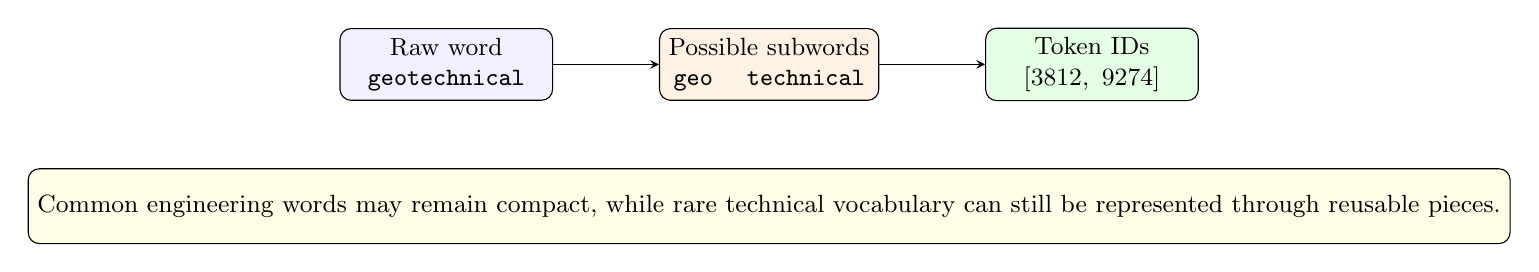
\begin{tikzpicture}[>=stealth,font=\small,x=1cm,y=1cm]
      \tikzset{box/.style={draw, rounded corners, minimum width=2.7cm, minimum height=0.8cm, align=center}}
      \node[box, fill=blue!6] (raw) at (0,0) {Raw word\\\texttt{geotechnical}};
      \node[box, fill=orange!10] (sub) at (4.1,0) {Possible subwords\\\texttt{geo} \quad \texttt{technical}};
      \node[box, fill=green!10] (ids) at (8.2,0) {Token IDs\\$[3812,\ 9274]$};
      \draw[->] (raw) -- (sub);
      \draw[->] (sub) -- (ids);
      \node[box, fill=yellow!10, minimum width=8.8cm, minimum height=0.95cm] at (4.1,-1.8)
        {Common engineering words may remain compact, while rare technical vocabulary can still be represented through reusable pieces.};
    \end{tikzpicture}
    \caption{Subword tokenization of a technical term.}
  \end{figure}
\end{frame}

\begin{frame}{Why Tokenization Matters in Engineering}
  A phrase like ``ACI 318 load combination'' contains:
  \begin{itemize}
    \item ordinary English,
    \item a code identifier,
    \item domain-specific technical terminology.
  \end{itemize}

  \begin{examplebox}{Practical Consequence}
    Tokenization affects cost, context-window usage, and sometimes output quality, especially in code-heavy or standards-heavy workflows.
  \end{examplebox}
\end{frame}

\section{From Tokens to Vectors}

\begin{frame}{What an Embedding Is}
  Each token is mapped to a vector of real numbers called an \textbf{embedding}.

  If vocabulary size is $|\mathcal{V}|$ and embedding dimension is $d$, then the embedding table is:
  \[
    E \in \mathbb{R}^{|\mathcal{V}|\times d}.
  \]

  Looking up a token returns one row of this matrix.

  \source{\href{https://en.wikipedia.org/wiki/Word_embedding}{Wikipedia: Word Embedding}}
\end{frame}

\begin{frame}{Token versus Embedding}
  \begin{conceptbox}{Definition}
    A token is a discrete symbol. An embedding is its continuous numerical representation.
  \end{conceptbox}

  Tokenization discretizes language.

  Embeddings place that language in a vector space where similarity can be computed.
\end{frame}

\begin{frame}{Why High-Dimensional Spaces Matter}
  Embeddings often live in hundreds or thousands of dimensions.

  This makes it possible to encode many weak signals simultaneously:
  \begin{itemize}
    \item syntax,
    \item topic,
    \item domain,
    \item tone,
    \item contextual association.
  \end{itemize}

  Cosine similarity is a common comparison measure:
  \[
    \mathrm{cos\_sim}(\mathbf{u},\mathbf{v}) = \frac{\mathbf{u}^\top\mathbf{v}}{\|\mathbf{u}\|\,\|\mathbf{v}\|}.
  \]
\end{frame}

\begin{frame}{Embedding Space as Geometry}
  \begin{figure}
    \centering
    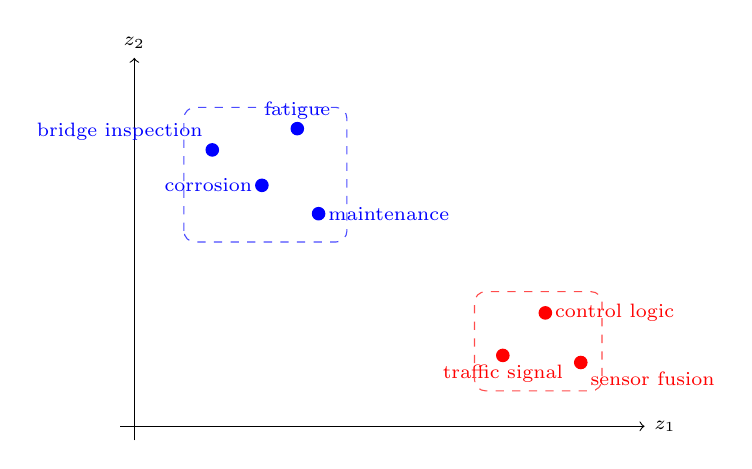
\begin{tikzpicture}[scale=0.9, every node/.style={font=\scriptsize}]
      \draw[->] (-0.2,0) -- (7.2,0) node[right] {$z_1$};
      \draw[->] (0,-0.2) -- (0,5.2) node[above] {$z_2$};
      \filldraw[blue] (1.1,3.9) circle (2.5pt) node[above left] {bridge inspection};
      \filldraw[blue] (1.8,3.4) circle (2.5pt) node[left] {corrosion};
      \filldraw[blue] (2.3,4.2) circle (2.5pt) node[above] {fatigue};
      \filldraw[blue] (2.6,3.0) circle (2.5pt) node[right] {maintenance};
      \filldraw[red] (5.2,1.0) circle (2.5pt) node[below] {traffic signal};
      \filldraw[red] (5.8,1.6) circle (2.5pt) node[right] {control logic};
      \filldraw[red] (6.3,0.9) circle (2.5pt) node[below right] {sensor fusion};
      \draw[dashed, rounded corners, blue!70] (0.7,2.6) rectangle (3.0,4.5);
      \draw[dashed, rounded corners, red!70] (4.8,0.5) rectangle (6.6,1.9);
    \end{tikzpicture}
    \caption{Low-dimensional view of embedding-space clustering.}
  \end{figure}
\end{frame}

\begin{frame}{Why the Geometry Is Useful}
  The point of the figure is not that embeddings are really two-dimensional.

  \begin{conceptbox}{Geometric Intuition}
    Semantically related items tend to lie near one another in the embedding space, even when the wording is not identical.
  \end{conceptbox}

  That is why a query about ``steel design loads'' can retrieve passages phrased as ``load combinations for structural steel members.''
\end{frame}

\begin{frame}{Front-End Representation Pipeline}
  \begin{figure}
    \centering
    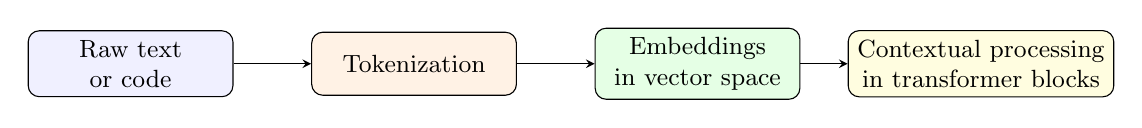
\begin{tikzpicture}[>=stealth,font=\small]
      \tikzset{box/.style={draw, rounded corners, minimum width=2.6cm, minimum height=0.8cm, align=center}}
      \node[box, fill=blue!6] (text) at (0,0) {Raw text\\or code};
      \node[box, fill=orange!10] (tok) at (3.6,0) {Tokenization};
      \node[box, fill=green!10] (emb) at (7.2,0) {Embeddings\\in vector space};
      \node[box, fill=yellow!12] (ctx) at (10.8,0) {Contextual processing\\in transformer blocks};
      \draw[->] (text) -- (tok);
      \draw[->] (tok) -- (emb);
      \draw[->] (emb) -- (ctx);
    \end{tikzpicture}
    \caption{Front-end representation pipeline for an LLM.}
  \end{figure}

  Topic 15 emphasizes the first half of this pipeline: how text becomes vectors.
\end{frame}

\begin{frame}{Sentence and Document Embeddings}
  In engineering workflows, we often compare larger units than single tokens:
  \begin{itemize}
    \item sentences,
    \item paragraphs,
    \item code blocks,
    \item report sections,
    \item table descriptions.
  \end{itemize}

  Conceptually, one simple aggregation idea is:
  \[
    \mathbf{s}=\frac{1}{m}\sum_{i=1}^{m}\mathbf{e}_i.
  \]
\end{frame}

\begin{frame}{Chunking Choices for Engineering Documents}
  \begin{tabular}{p{0.42\textwidth} p{0.44\textwidth}}
    \toprule
    \textbf{Source material} & \textbf{Possible chunk} \\
    \midrule
    Design code PDF & one clause or paragraph \\
    Structural report & one subsection or executive-summary paragraph \\
    Spreadsheet note export & one row with neighboring notes \\
    Python script & one function or docstring-plus-function block \\
    Inspection log & one observation entry \\
    \bottomrule
  \end{tabular}

  Chunking matters because fragments that are too small lose meaning, while chunks that are too large become noisy and expensive.
\end{frame}

\section{Vector Stores and Retrieval}

\begin{frame}{What a Vector Store Does}
  Once documents or code blocks are converted into embeddings, those vectors can be stored and searched.

  \begin{conceptbox}{Vector Store}
    A vector store is a database or indexing system designed to store numerical embeddings together with metadata and original text.
  \end{conceptbox}
\end{frame}

\begin{frame}{Basic Retrieval Pipeline}
  The basic pipeline is straightforward:
  \begin{enumerate}
    \item split documents into chunks,
    \item embed each chunk as a vector,
    \item store vector + metadata + original text,
    \item embed the user query,
    \item retrieve nearby vectors,
    \item return the associated human-readable chunks.
  \end{enumerate}

  \source{\href{https://arxiv.org/abs/2005.11401}{Lewis et al. (2020): Retrieval-Augmented Generation}}
\end{frame}

\begin{frame}{Similarity Search}
  Suppose a query embedding is $\mathbf{q}$ and stored chunk embeddings are $\mathbf{v}_1,\dots,\mathbf{v}_N$.

  A simple retrieval score is:
  \[
    s_i = \mathrm{cos\_sim}(\mathbf{q},\mathbf{v}_i)
  \]

  and the system returns the top-$k$ chunks:
  \[
    \mathcal{R}_k(\mathbf{q}) = \operatorname{TopK}_{i=1,\dots,N}\ s_i.
  \]

  In production, systems often use approximate nearest-neighbor indexing, reranking, or hybrid retrieval.
\end{frame}

\begin{frame}{Keyword Search versus Semantic Search}
  \small
  \begin{tabular}{p{0.25\textwidth} p{0.29\textwidth} p{0.29\textwidth}}
    \toprule
    \textbf{Query type} & \textbf{Keyword search strong when} & \textbf{Semantic search strong when} \\
    \midrule
    Exact clause lookup & exact citation known & wording varies \\
    Prior project search & terminology repeated & ideas paraphrased \\
    Spreadsheet lookup & labels exact & assumptions in prose \\
    Research support & proper nouns matter & concept similarity matters \\
    \bottomrule
  \end{tabular}

  In engineering, hybrid retrieval is often the natural choice.
\end{frame}

\begin{frame}{How Does a Sentence Come Back?}
  A vector store does not store meaning in ordinary words alone.

  Each stored item looks conceptually like:
  \begin{tabular}{llll}
    \toprule
    ID & Vector & Source metadata & Original text \\
    \midrule
    17 & $\mathbf{v}_{17}$ & Report A, p.
    42 & ``Deflection under service load shall...'' \\
    18 & $\mathbf{v}_{18}$ & Report B, p.
    11 & ``Load combinations for steel beams...'' \\
    \bottomrule
  \end{tabular}

  The vector is the search key; the original text remains the payload shown to the user.
\end{frame}

\begin{frame}{Nearest-Neighbor Retrieval as Geometry}
  \begin{figure}
    \centering
    \begin{tikzpicture}[scale=0.9, every node/.style={font=\scriptsize}]
      \draw[->] (-0.2,0) -- (7.2,0) node[right] {$z_1$};
      \draw[->] (0,-0.2) -- (0,5.2) node[above] {$z_2$};
      \filldraw[blue] (1.5,4.1) circle (2.5pt) node[above] {chunk 17};
      \filldraw[blue] (2.2,3.6) circle (2.5pt) node[left] {chunk 18};
      \filldraw[blue] (1.8,2.9) circle (2.5pt) node[left] {chunk 24};
      \filldraw[blue] (5.7,1.4) circle (2.5pt) node[right] {chunk 52};
      \filldraw[blue] (6.1,2.0) circle (2.5pt) node[right] {chunk 53};
      \filldraw[red] (1.9,3.8) circle (3pt) node[above right] {query};
      \draw[thick, red, dashed] (1.9,3.8) circle (0.7);
      \draw[->, thick, red] (1.9,3.8) -- (1.55,4.05);
      \draw[->, thick, red] (1.9,3.8) -- (2.15,3.62);
    \end{tikzpicture}
    \caption{Nearest-neighbor retrieval in an embedding space.}
  \end{figure}
\end{frame}

\begin{frame}{Why the Retrieval Figure Matters}
  The retrieval picture shows three key ideas:
  \begin{itemize}
    \item the query is embedded into the same vector space as stored chunks,
    \item retrieval returns nearby chunk IDs rather than ``meaning'' directly,
    \item metadata and original text are required to recover usable engineering evidence.
  \end{itemize}

  \source{\href{https://github.com/facebookresearch/faiss}{FAISS: similarity search and clustering}}
\end{frame}

\begin{frame}{A Small Numerical Example}
  Suppose the query is
  \[
    q = \texttt{"serviceability limit for beam deflection"}
  \]

  and the similarities are:
  \begin{itemize}
    \item ``Deflection under service loads shall remain within specified limits.'' $\rightarrow 0.92$
    \item ``Ultimate strength combinations control flexural resistance.'' $\rightarrow 0.67$
    \item ``Retaining wall drainage layers reduce pore pressure.'' $\rightarrow 0.18$
  \end{itemize}

  The top result is semantically relevant even if the exact phrase ``beam deflection'' is absent.
\end{frame}

\begin{frame}{Why Metadata Matters}
  Metadata is the bridge back to the engineering source of truth.

  Engineers usually need to know:
  \begin{itemize}
    \item which document the chunk came from,
    \item what page or section it belongs to,
    \item whether the source is current, approved, or superseded,
    \item whether it came from a code, report, note, or codebase.
  \end{itemize}

  Without metadata, semantic similarity alone does not support traceability or auditability.
\end{frame}

\section{Generation Limits: Hallucination and Reliability}

\begin{frame}{What Hallucination Means}
  In this context, a hallucination is output that is:
  \begin{itemize}
    \item fluent,
    \item plausible,
    \item but unsupported, incorrect, fabricated, or overconfident.
  \end{itemize}

  \begin{warningbox}{Engineering Interpretation}
    An LLM is optimized to continue text plausibly, not to guarantee truth in the strict engineering sense.
  \end{warningbox}

  \source{\href{https://en.wikipedia.org/wiki/Hallucination_(artificial_intelligence)}{Wikipedia: Hallucination (artificial intelligence)}}
\end{frame}

\begin{frame}{Why Hallucinations Occur}
  Several mechanisms contribute:
  \begin{itemize}
    \item probabilistic next-token generation,
    \item incomplete context,
    \item post-training pressure to be helpful,
    \item distribution shift on specialized technical questions,
    \item decoding choices.
  \end{itemize}

  This explains why a model may sound confident when it should instead say, ``I need the source document.''
\end{frame}

\begin{frame}{Temperature and Output Reliability}
  Temperature scaling changes how aggressively the model explores alternatives:
  \[
    P_T(v) \propto \exp\!\left(\frac{\log P(v)}{T}\right)
  \]

  \small
  \begin{tabular}{lll}
    \toprule
    \textbf{Temperature} & \textbf{Behavior} & \textbf{Typical use} \\
    \midrule
    Low ($0$--$0.3$) & focused, low variance & coding, factual QA \\
    Medium ($0.4$--$0.7$) & balanced & analysis, summarization \\
    High ($0.8+$) & exploratory & brainstorming \\
    \bottomrule
  \end{tabular}
\end{frame}

\begin{frame}{Lower Temperature Is Not a Cure}
  \begin{warningbox}{Important Limitation}
    Lower temperature may reduce some variation, but it does not solve missing knowledge, weak retrieval, or poor calibration. A deterministic wrong answer is still wrong.
  \end{warningbox}

  This is why reliability must be designed into the workflow, not delegated to one decoding setting.
\end{frame}

\begin{frame}{How Engineers Should Respond}
  In engineering settings, hallucination risk should be reduced by:
  \begin{itemize}
    \item grounding answers in retrieved documents or cited standards,
    \item using lower-variance decoding for factual tasks,
    \item asking for assumptions, sources, and intermediate checks,
    \item treating outputs as drafts rather than final truth,
    \item keeping a human reviewer in the loop.
  \end{itemize}
\end{frame}

\section{Conclusion and Transition}

\begin{frame}{Putting the Pieces Together}
  The document-retrieval pipeline that connects LLMs to engineering knowledge work is:
  \begin{enumerate}
    \item split technical documents into chunks,
    \item convert each chunk into an embedding,
    \item store vectors and metadata in a searchable index,
    \item embed the query into the same space,
    \item retrieve nearby vectors,
    \item return the original text chunks for synthesis or review.
  \end{enumerate}
\end{frame}

\begin{frame}{Chapter Takeaways}
  \begin{itemize}
    \item LLMs matter in engineering because engineering work is document-heavy.
    \item NLP historically struggled with both representation and scale.
    \item Transformers, pretraining, and large-scale compute changed the field.
    \item Tokenization and embeddings are the bridge from text to computation.
    \item Vector retrieval makes meaning-based document search practical.
    \item Hallucination remains a serious limitation and requires human oversight.
  \end{itemize}
\end{frame}

\begin{frame}{From Topic 15 to Topic 16}
  Topic 15 focused on motivation and representation.

  Topic 16 will build on this foundation by asking:
  \begin{itemize}
    \item how modern LLM systems are organized internally,
    \item how prompting and workflow design change engineering practice,
    \item how retrieval, knowledge engineering, and agentic systems extend the base model.
  \end{itemize}

  That discussion will naturally lead toward Topic 17 and human-in-the-loop engineering.
\end{frame}

\end{document}
